\documentclass[10pt]{beamer}

\usetheme{Frankfurt}

%%% Работа с русским языком
\usepackage{cmap}					% поиск в PDF
\usepackage{mathtext} 				% русские буквы в формулах
\usepackage[T2A]{fontenc}			% кодировка
\usepackage[utf8]{inputenc}			% кодировка исходного текста
\usepackage[english,russian]{babel}	% локализация и переносы
\usepackage{indentfirst}
\frenchspacing


%%% Дополнительная работа с математикой
\usepackage{amsmath,amsfonts,amssymb,amsthm,mathtools} % AMS
\usepackage{icomma} % "Умная" запятая: $0,2$ --- число, $0, 2$ --- перечисление

%% Номера формул
%\mathtoolsset{showonlyrefs=true} % Показывать номера только у тех формул, на которые есть \eqref{} в тексте.
%\usepackage{leqno} % Нумерация формул слева

%% Свои команды
\DeclareMathOperator{\sgn}{\mathop{sgn}}

%% Перенос знаков в формулах (по Львовскому)
\newcommand*{\hm}[1]{#1\nobreak\discretionary{}
	{\hbox{$\mathsurround=0pt #1$}}{}}

%%% Работа с картинками
\usepackage{graphicx}  % Для вставки рисунков
\graphicspath{{images/}}  % папки с картинками
\setlength\fboxsep{3pt} % Отступ рамки \fbox{} от рисунка
\setlength\fboxrule{1pt} % Толщина линий рамки \fbox{}
\usepackage{wrapfig} % Обтекание рисунков текстом
\usepackage{subfigure}

%%% Работа с таблицами
\usepackage{array,tabularx,tabulary,booktabs} % Дополнительная работа с таблицами
\usepackage{longtable}  % Длинные таблицы
\usepackage{multirow} % Слияние строк в таблице

%%% Программирование
\usepackage{etoolbox} % логические операторы

%
%\usepackage{fancyhdr} % Колонтитулы
% 	\pagestyle{fancy}
%\renewcommand{\headrulewidth}{0pt}  % Толщина линейки, отчеркивающей верхний колонтитул
% 	\lfoot{Нижний левый}
% 	\rfoot{Нижний правый}
% 	\rhead{Верхний правый}
% 	\chead{Верхний в центре}
% 	\lhead{Верхний левый}
%	\cfoot{Нижний в центре} % По умолчанию здесь номер страницы

\usepackage{setspace} % Интерлиньяж
%\onehalfspacing % Интерлиньяж 1.5
%\doublespacing % Интерлиньяж 2
%\singlespacing % Интерлиньяж 1

\usepackage{lastpage} % Узнать, сколько всего страниц в документе.

\usepackage{soul} % Модификаторы начертания


\usepackage{csquotes} % Еще инструменты для ссылок

%\usepackage[style=authoryear,maxcitenames=2,backend=biber,sorting=nty]{biblatex}

\usepackage{multicol} % Несколько колонок

\usepackage{tikz} % Работа с графикой
\usepackage{pgfplots}
\usepackage{pgfplotstable}

\renewcommand{\phi}{\varphi}
\renewcommand{\epsilon}{\varepsilon}
\usepackage[justification=centering, font=footnotesize]{caption}
\setbeamertemplate{caption}[numbered]

\setlength{\parskip}{0.1cm}

\author{Кирилл Сёмкин \and Денис Швейкин \and Александр Савельев \\ Александр Богданов \and Евгений Рябинин}
\date{Математика больших данных, 2023}
\title{Возникновение пробок и явление фазового перехода в системах массового обслуживания}

\begin{document}
	
	\begin{frame}[c]
		\titlepage
	\end{frame}
	
	\begin{frame}{Задача о кассе в час пик}
		
		\textbf{Постановка} 
		
		\only<1>{
			Люди подходят к кассе с интенсивностью $ \phi(t) $ - монотонно неубывающей со временем; кассир обслуживает людей с постоянной интенсивностью $ \lambda $. Ставится вопрос: насколько быстро будет меняться среднее число людей в очереди? Поняв это, можно, например, предсказывать через сколько времени придётся открыть вторую кассу и решать другие прикладные задачи.
			
			В терминах непрерывных марковских цепей имеем следующую модель, см. рис.\ref{pic:mark_chain}. 
		}
		
		\only<2>{
			В данном случае цепь не является однородной. Тем не менее динамика переходов будет похожей на классический случай:
			
			\begin{center}
				$
				\begin{cases*}
					\dot{P}(t) = Q(t) \cdot P(t) \\
					P(0) = I
				\end{cases*} \Rightarrow
				$ 
				$
				\begin{cases*}
					\dot{\pi}(t) = \dot{P}(t) \pi(0) = Q(t) \pi(t) \\
					\pi(0) = \pi^0
				\end{cases*}
				$
			\end{center}
			
			% TODO сказать здесь, что по хорошему N нужно устремлять к бесконечности
		}
		
		\begin{figure}
			\centering
			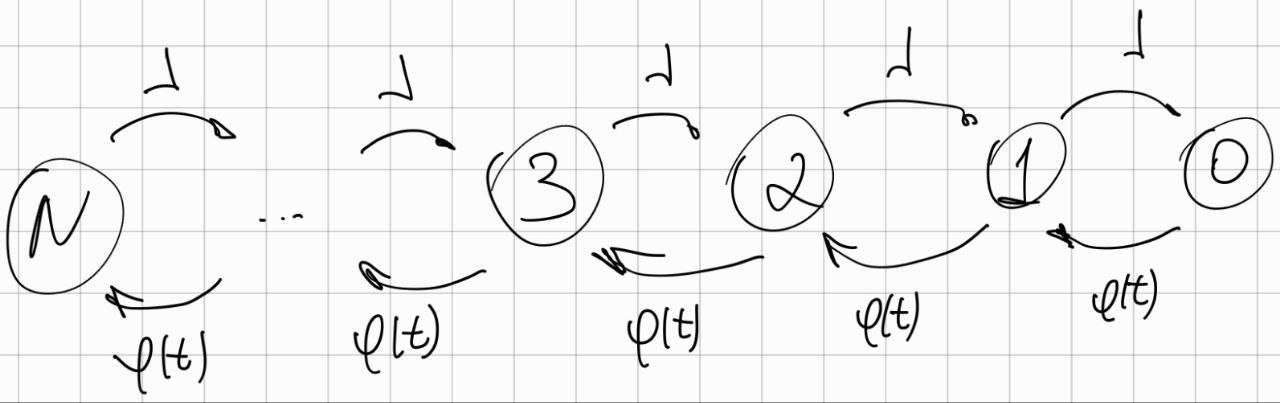
\includegraphics[width=0.5\textwidth, keepaspectratio]{../img/mark_chain}
			\caption{Марковская цепь задачи}\label{pic:mark_chain}
		\end{figure}
		
	\end{frame}
	
	\begin{frame}{Уравнения динамики цепи}
		
		Т.о. имеем следующие уравнения динамики:
		
		\begin{gather*}
			\dot{\pi}_0 = - \phi(t) \pi_0 + \lambda \pi_1 \\
			\dot{\pi}_1 = \lambda \pi_2 + \phi(t) \pi_0 - (\lambda + \phi(t)) \pi_1 \\
			\dot{\pi}_2 = \lambda \pi_3 + \phi(t) \pi_1 - (\lambda + \phi(t)) \pi_2 \\
			\ldots \\
			\dot{\pi}_N = \phi(t) \pi_{N-1} - \lambda \pi_N		
		\end{gather*}\label{eq:dinamics}
		
		При этом одно уравнение формально лишнее, т.к. $ \sum \pi_i(t) = 1 \Rightarrow \sum \dot{\pi}_i(t) = 0 $
		
		% TODO сказать здесь, что система сложная даже с простыми phi(t), т.к. каждое сосотяние получается связанным с каждым другим
		
		\pause
		
		Нас интересует поведение $ \mathbb{E}[S](t) = \sum\limits_{k = 0}^N \pi_k k \Rightarrow \frac{d}{dt} \mathbb{E}[S](t) = \sum\limits_{k = 0}^N \dot{\pi}_k k $, где $ S(t) $ --- состояние цепи (кол-во людей в очереди) в момент $ t $.
		
	\end{frame}
	
	\begin{frame}{Случай постоянного потока}
		
		Пусть $ \phi(t) = \mu = const $, тогда имеем простую цепь гибели/рождения. Данная цепь является эргодической, со стационарным распределением $ \tilde{\pi} $:
		
		\[
			\tilde{\pi}_j = \frac{\mu}{\lambda} \tilde{\pi}_{j-1} \Rightarrow \tilde{\pi}_j = (\frac{\mu}{\lambda})^j \cdot \tilde{\pi}_0 
		\]
		
		\pause
		
		Введём обозначение $ q = \mu / \lambda $. Используя $ \sum \pi_i = 1 $, получим:
		
		\[
			\tilde{\pi}_0 = \frac{q - 1}{q^{N + 1} - 1}
		\]		
		
	\end{frame}
	
	\begin{frame}{Случай постоянного потока}
		
		\only<1>{
			Т.о. при заданном $ N $ имеем дискретное экспоненциальное распределение на числе людей в очереди: при $ q > 1 $ вероятности больше для большего людей в очереди, при $ q < 1 $ - наоборот (при $ q = 1 $ имеем равномерное распределение). Ниже представлены вид распределений для разных $ q $.
		}
		
		\only<2>{
			\begin{figure}
				\centering
				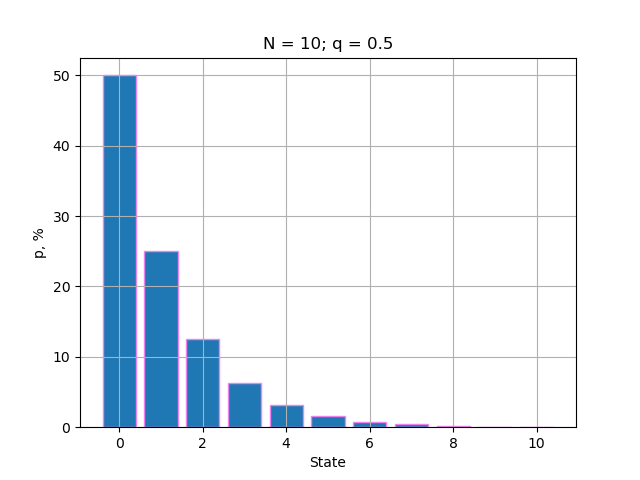
\includegraphics[width=0.48\textwidth, keepaspectratio]{../img/stationary_case/distr_0.png}
				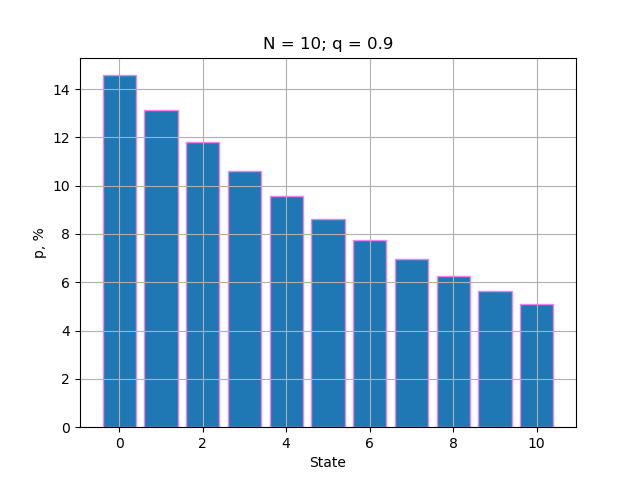
\includegraphics[width=0.48\textwidth, keepaspectratio]{../img/stationary_case/distr_1.png}
				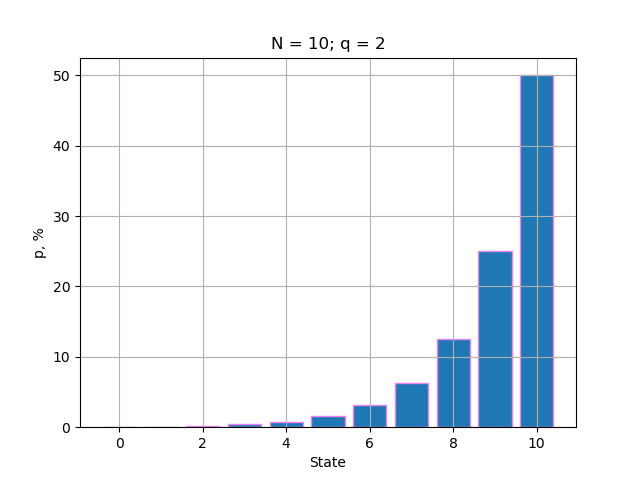
\includegraphics[width=0.48\textwidth, keepaspectratio]{../img/stationary_case/distr_2.png}
				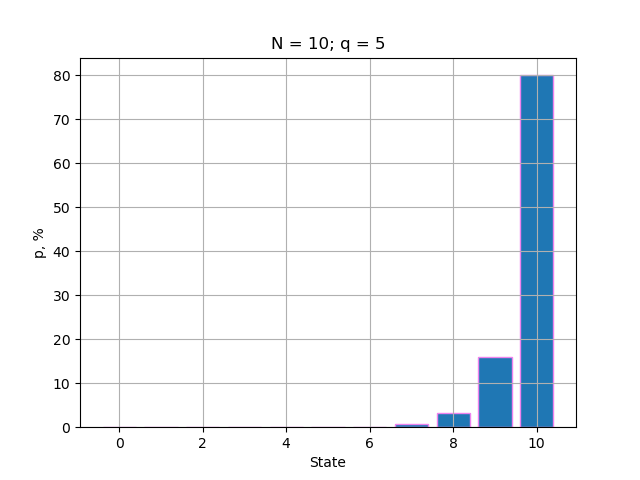
\includegraphics[width=0.48\textwidth, keepaspectratio]{../img/stationary_case/distr_3.png}
				\caption{Виды стационарных состояний цепи}\label{pic:stationary}
			\end{figure}
		}
		
	\end{frame}
	
	\begin{frame}{Случай постоянного потока}
		
		\only<1>{
			Вычислим среднее:
			
			\begin{equation*}
				\mathbb{E}[S](t) = \sum\limits_{k = 0}^N \pi_k k = \tilde{\pi}_0 \sum\limits_{k = 0}^N k q^k
			\end{equation*}
			
			При $ q < 1 $ можно воспользоваться приближением при $ N \gg 1 $:
			
			\begin{equation*}
				\mathbb{E}[S](t) = \tilde{\pi}_0 \sum\limits_{k = 0}^N k q^k \approx \tilde{\pi}_0 \sum\limits_{k = 0}^{\infty} k q^k = \tilde{\pi}_0 \frac{q}{(1 - q)^2}
			\end{equation*}
			
			При $ q > 1 $ можно воспользоваться оценкой через интеграл:
			
			\begin{multline*}
				\mathbb{E}[S](t) = \tilde{\pi}_0 \sum\limits_{k = 0}^N k q^k \approx \tilde{\pi}_0 \int\limits_{0}^N x \cdot q^x dx = \frac{1}{\log^2 q} (q^N (N \log q - 1) + 1) \sim \\ \sim q^N \cdot \frac{N}{\log q}
			\end{multline*}
			
		}
		
		\only<2>{
			Посмотрим на точные вычисленные значения средних при разных режимах $ q $:
			
			\begin{figure}
				\centering
				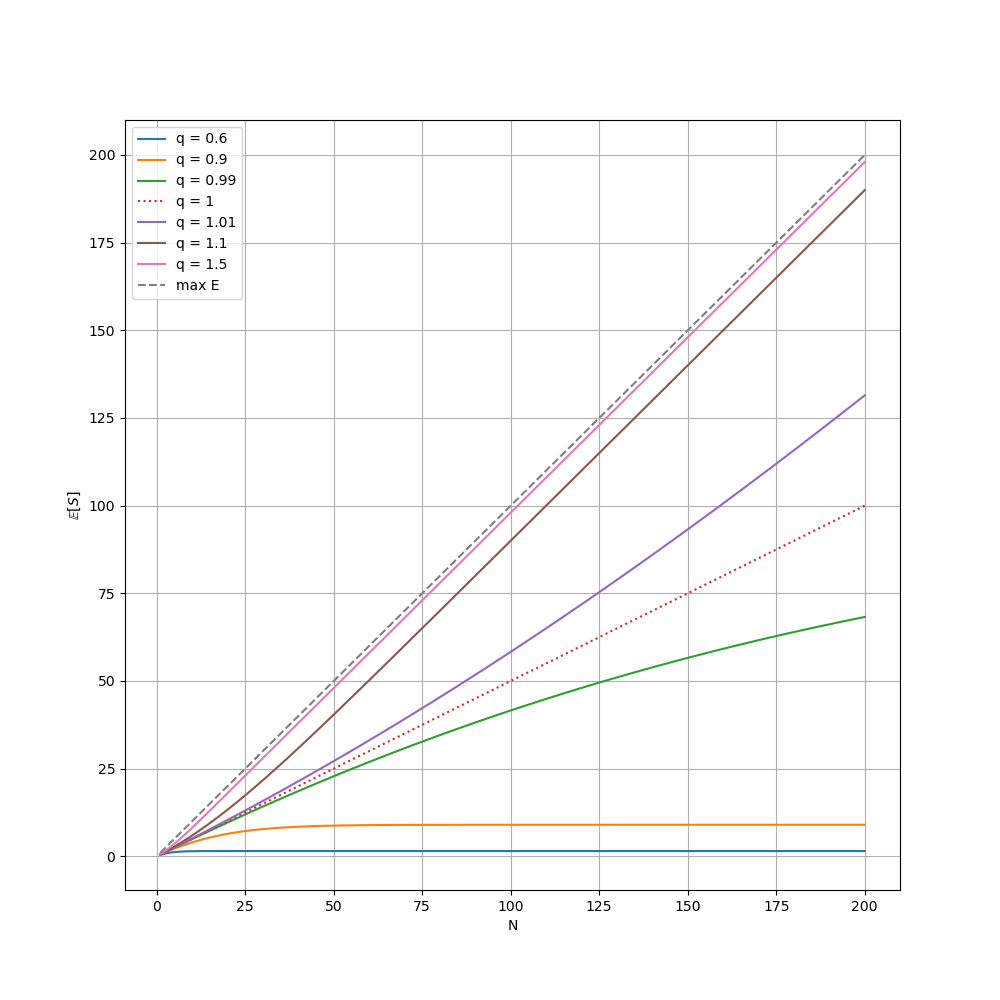
\includegraphics[width=0.6\textwidth, keepaspectratio]{../img/stationary_case/averages.png}
				\caption{Средний размер очереди при разных режимах}\label{pic:stationary_aver}
			\end{figure}
		}
		
		\only<3>{
			Видим фазовый переход с критической точкой $ q = 1 $.
			
			\begin{figure}
				\centering
				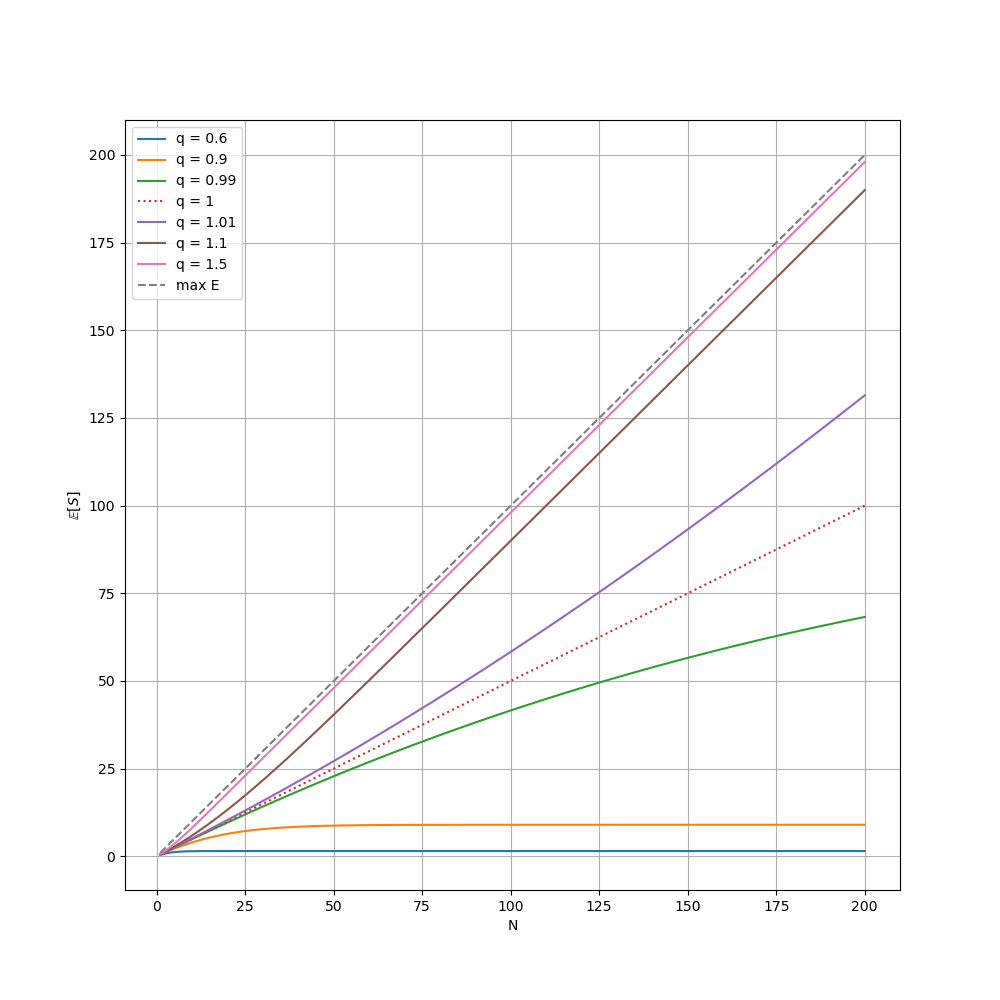
\includegraphics[width=0.6\textwidth, keepaspectratio]{../img/stationary_case/averages.png}
				\caption{Средний размер очереди при разных режимах}\label{pic:stationary_aver}
			\end{figure}
		}
		
	\end{frame}

	\begin{frame}{Приближение быстрого наплыва}
		
		\only<1>{
				Вернёмся к исходной задаче. Пусть $ |\phi(t)| \gg \lambda $ с самого начала $ t \ge 0 $. Тогда в уравнениях динамики можно пренебречь членами $ \lambda \cdot \pi_i $, т.е. пренебрегаем работай кассира и оцениваем насколько быстро будет расти очередь в первые моменты времени. В этом случае имеем цепь рис.\ref{pic:chain_surge} , т.е. неоднородный пуассоновский поток (считаем, что $ N $ может быть сколь угодно большим для простоты).
				
				\begin{figure}
					\centering
					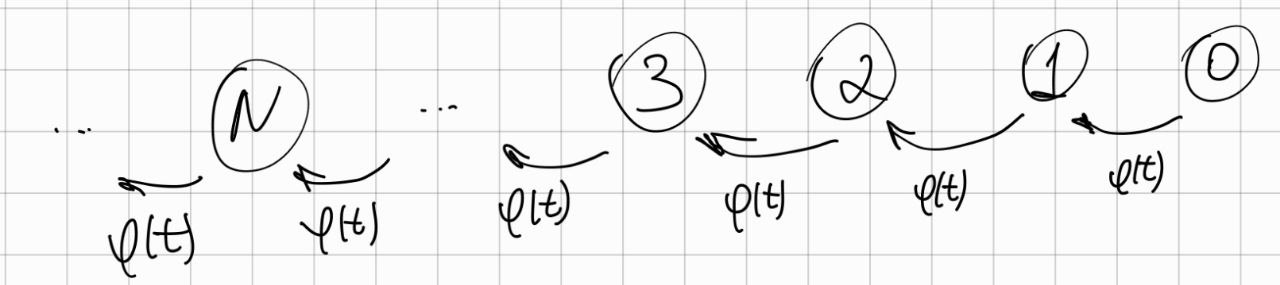
\includegraphics[width=0.6\textwidth, keepaspectratio]{../img/mark_chain_pois.jpg}
					\caption{Приближение цепи в начале наплыва}\label{pic:chain_surge}
				\end{figure}
		}
		
		\only<2>{
			Тогда кол-во людей в очереди распределено:
			
			\[
			S(t) \sim Po(\int_0^t \phi(s) ds) 
			\] 
			
			Со средним и дисперсией пуассоновской случайной величины, т.е.:
			
			\[
			\mathbb{E}[S(t)]  = \mathbb{D}[S(t)]= \int_0^t \phi(s) ds  
			\]
			
			\textbf{Примеры}
			
			\begin{itemize}
				\item $ \phi(s) \propto s^k \Rightarrow \mathbb{E}[S(t)] \propto s^{k + 1} $ 
				
				\item $ \phi(s) \propto e^s \Rightarrow \mathbb{E}[S(t)] \propto e^s $ 
			\end{itemize}
		}
		
	\end{frame}
	
	\begin{frame}{Численное решение}
		
		\only<1>{
			Теперь найдём точное решение уравнений динамики вероятностей $ \pi_i(t) $ численными методами в разных режимах интенсивностей. Для этого использовался метод Рунге-Кутты 4 порядка.
		}
		
		\only<2>{
			% TODO обращаем внимание на фазовый переход, он есть!
			
			\begin{figure}
				\centering
				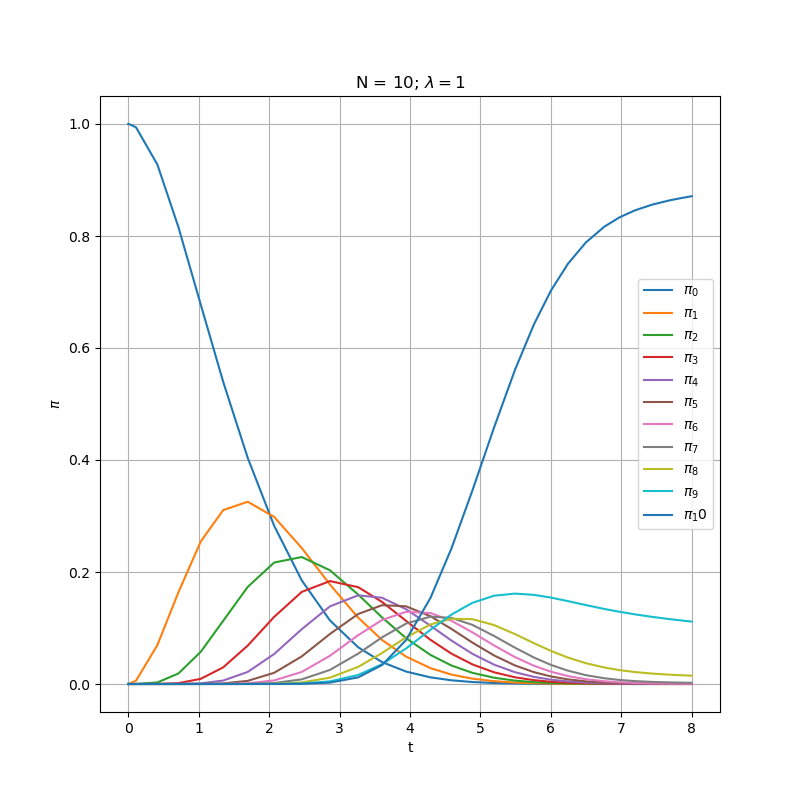
\includegraphics[width=0.48\textwidth, keepaspectratio]{../img/numeric_sol/probabilities_N_10_lambda_1_lin.png}
				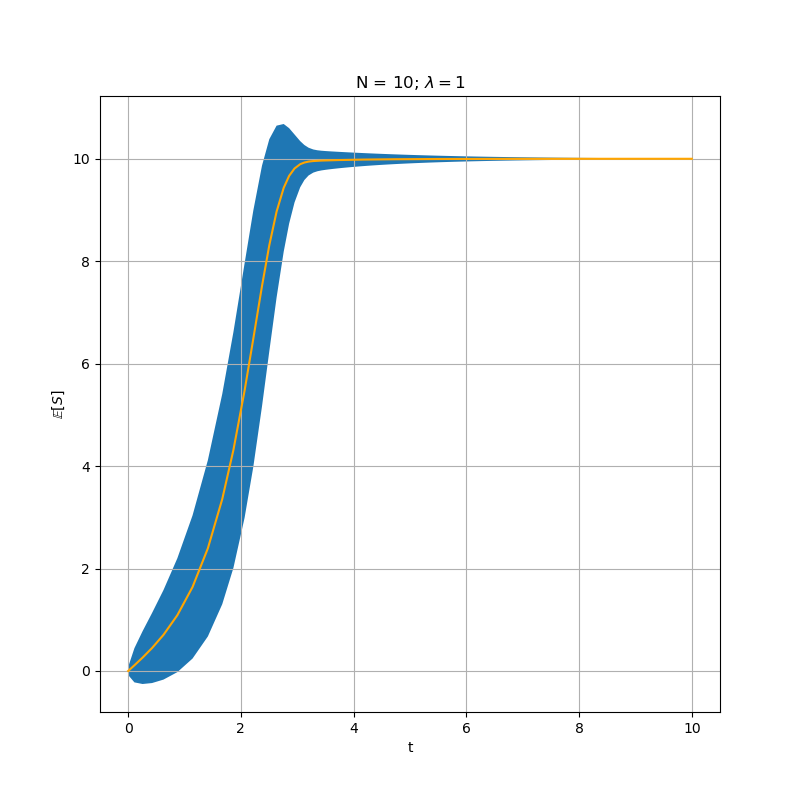
\includegraphics[width=0.48\textwidth, keepaspectratio]{../img/numeric_sol/avers_N_10_lambda_1_lin.png}
				\caption{Численные решения для $ \phi(t) = t $}
			\end{figure}
		}
		
		\only<3>{
			% TODO обращаем внимание на фазовый переход, он есть!
			
			\begin{figure}
				\centering
				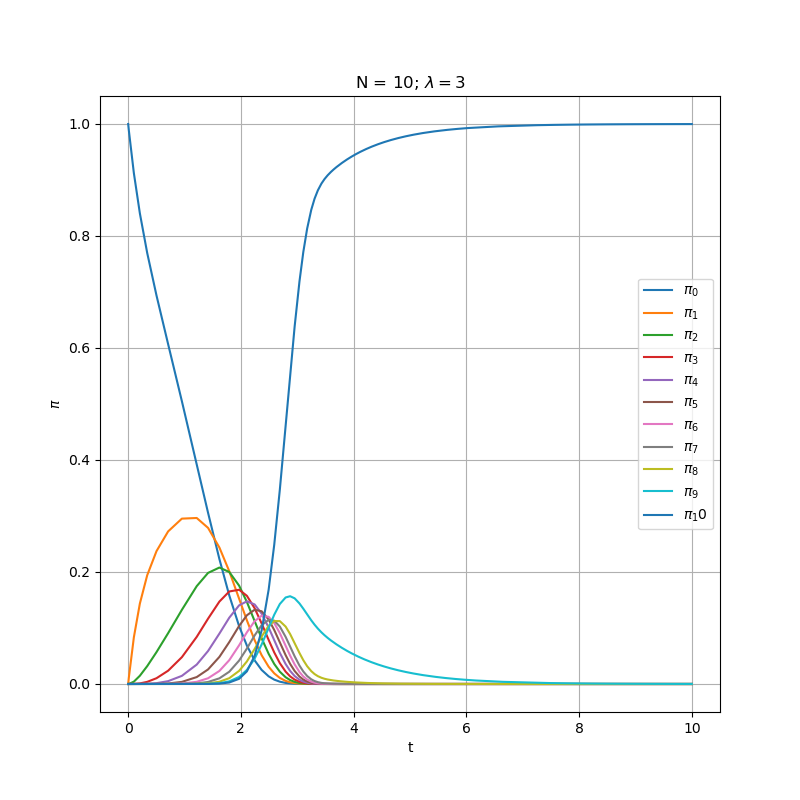
\includegraphics[width=0.48\textwidth, keepaspectratio]{../img/numeric_sol/probabilities_N_10_lambda_3_lin.png}
				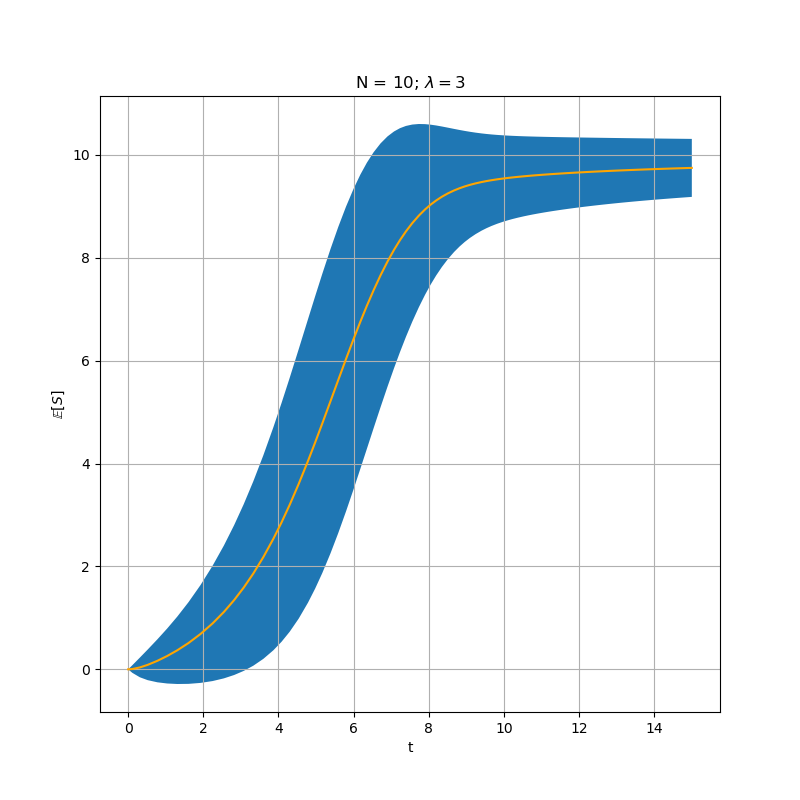
\includegraphics[width=0.48\textwidth, keepaspectratio]{../img/numeric_sol/avers_N_10_lambda_3_lin.png}
				\caption{Численные решения для $ \phi(t) = t $}
			\end{figure}
		}
		
		\only<4>{
			% TODO обращаем внимание на фазовый переход, он есть!
			
			\begin{figure}
				\centering
				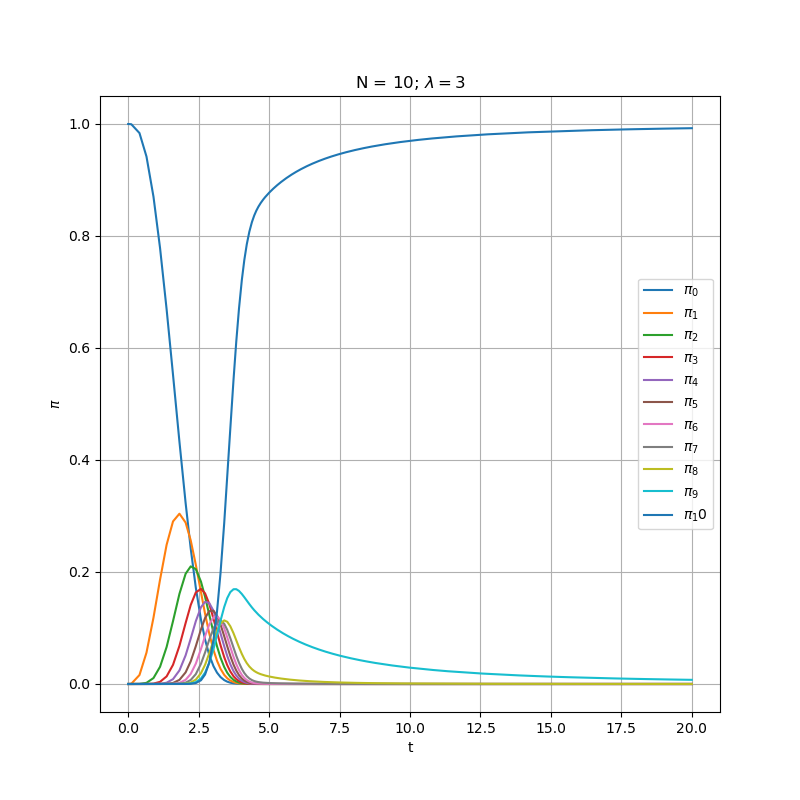
\includegraphics[width=0.48\textwidth, keepaspectratio]{../img/numeric_sol/probabilities_N_10_lambda_3_poly.png}
				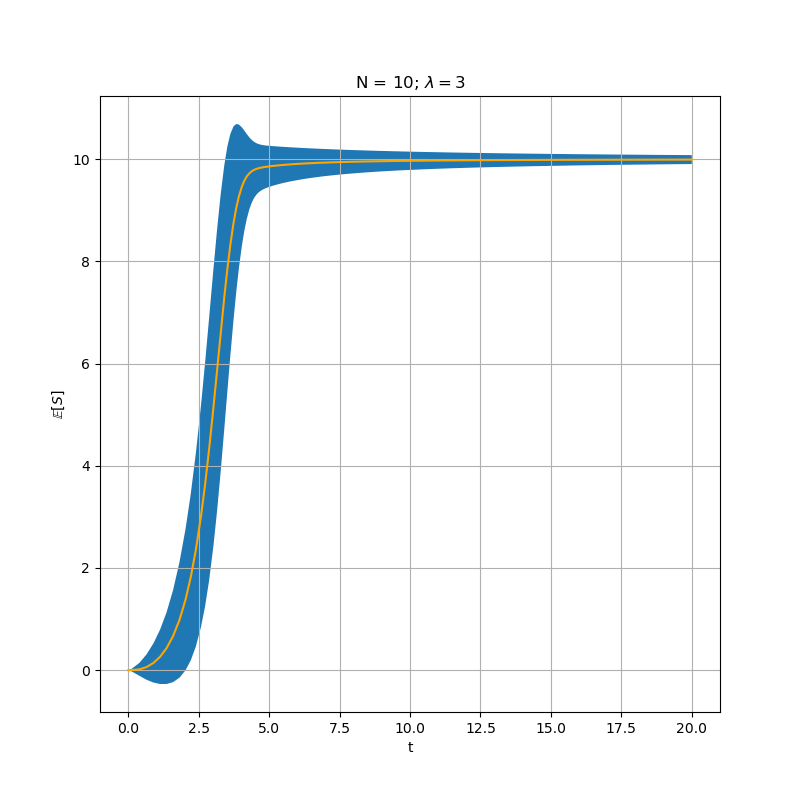
\includegraphics[width=0.48\textwidth, keepaspectratio]{../img/numeric_sol/avers_N_10_lambda_3_poly.png}
				\caption{Численные решения для $ \phi(t) = t^2 $}
			\end{figure}
		}
		
		\only<5>{
			% TODO обращаем внимание на фазовый переход, он есть!
			
			\begin{figure}
				\centering
				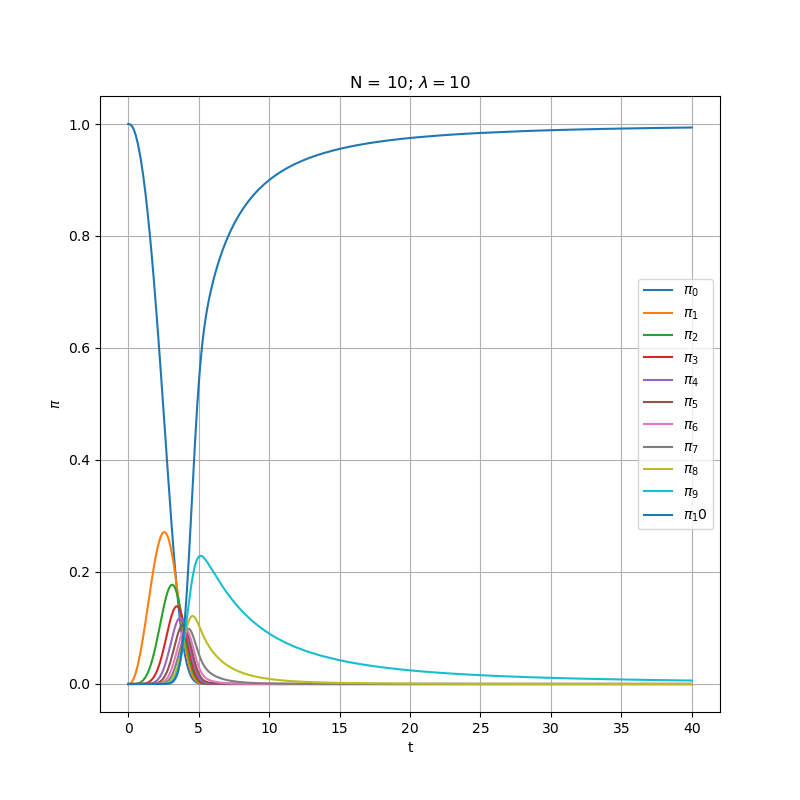
\includegraphics[width=0.48\textwidth, keepaspectratio]{../img/numeric_sol/probabilities_N_10_lambda_10_poly.png}
				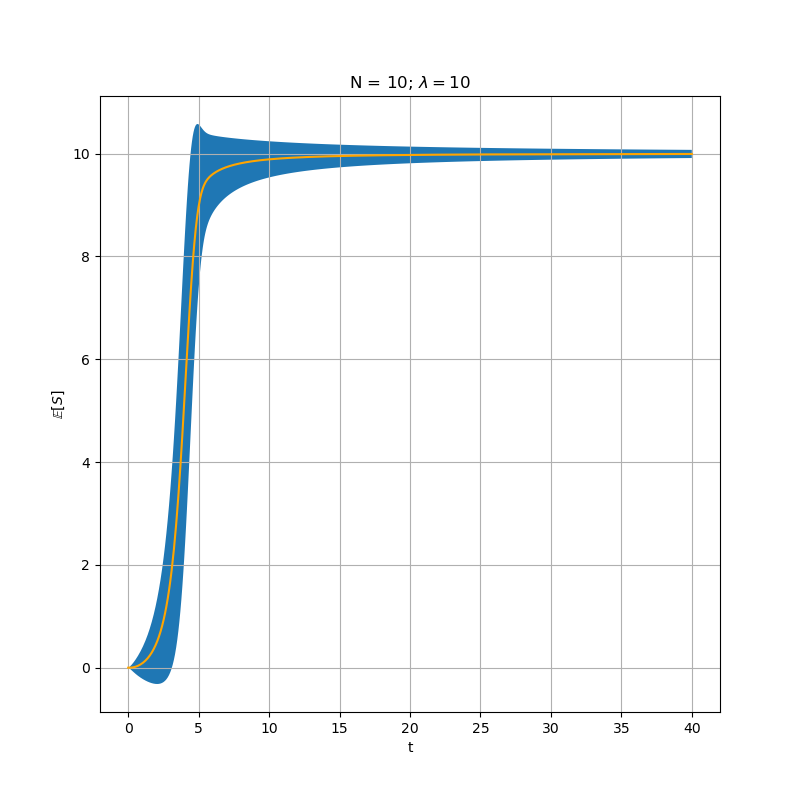
\includegraphics[width=0.48\textwidth, keepaspectratio]{../img/numeric_sol/avers_N_10_lambda_10_poly.png}
				\caption{Численные решения для $ \phi(t) = t^2 $}
			\end{figure}
		}
		
		\only<6>{
			% TODO обращаем внимание на фазовый переход, он есть!
			
			\begin{figure}
				\centering
				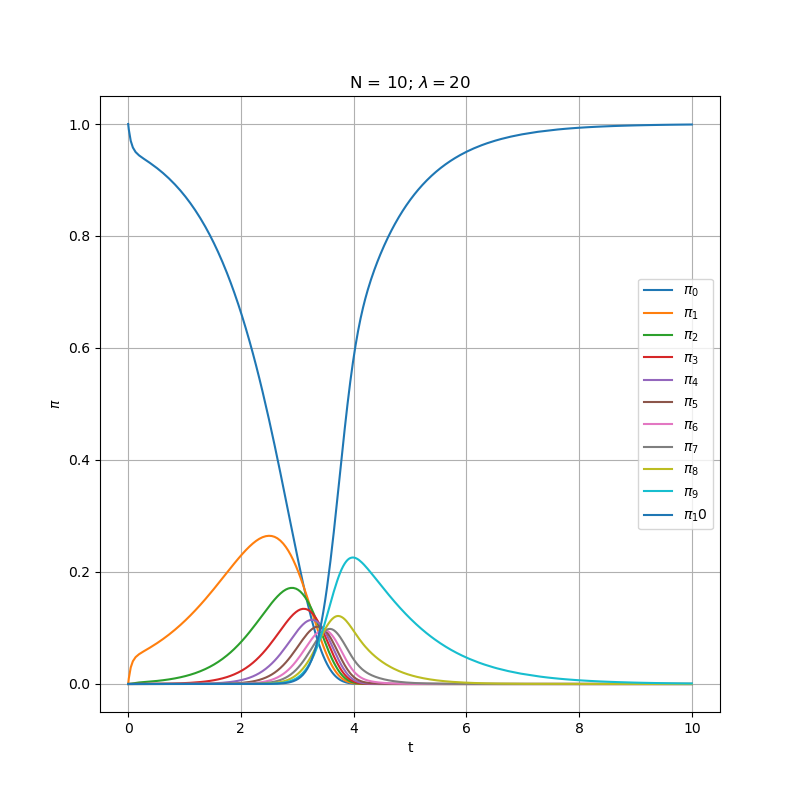
\includegraphics[width=0.48\textwidth, keepaspectratio]{../img/numeric_sol/probabilities_N_10_lambda_20_exp.png}
				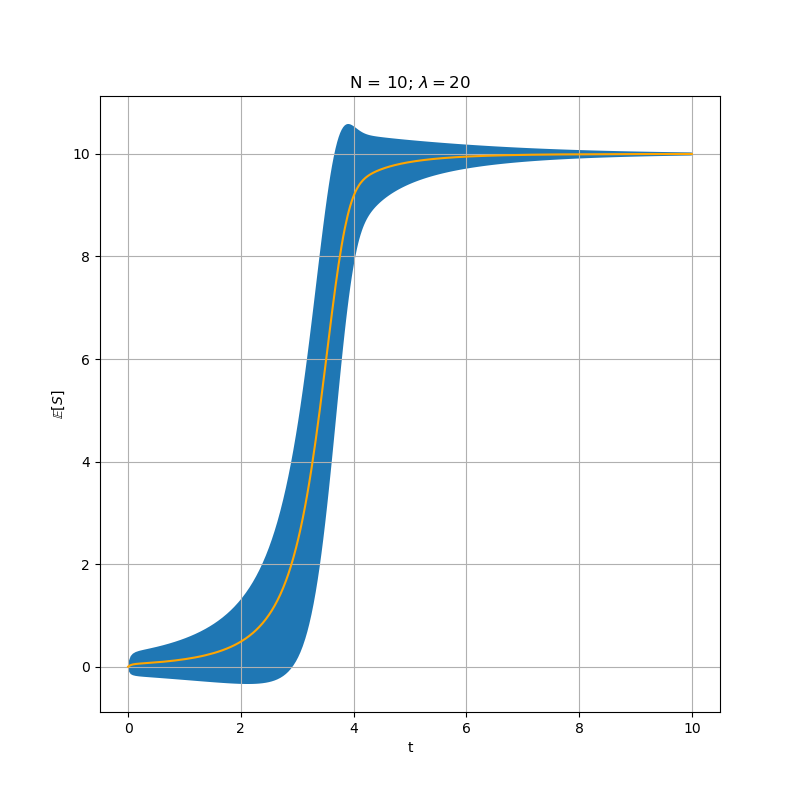
\includegraphics[width=0.48\textwidth, keepaspectratio]{../img/numeric_sol/avers_N_10_lambda_20_exp.png}
				\caption{Численные решения для $ \phi(t) = \exp(t) $}
			\end{figure}
		}
		
	\end{frame}
	
	\begin{frame}{Монте-Карло моделирование цепи}
		
		\only<1>{
			Вместо решения СОДУ можно просимулировать динамику цепи, сэмплируя случайные величины в дискретные моменты времени. Результаты совпадают с полученными выше.
		}
		
		\only<2>{
			% TODO обращаем внимание на фазовый переход, он есть!
			
			\begin{figure}
				\centering
				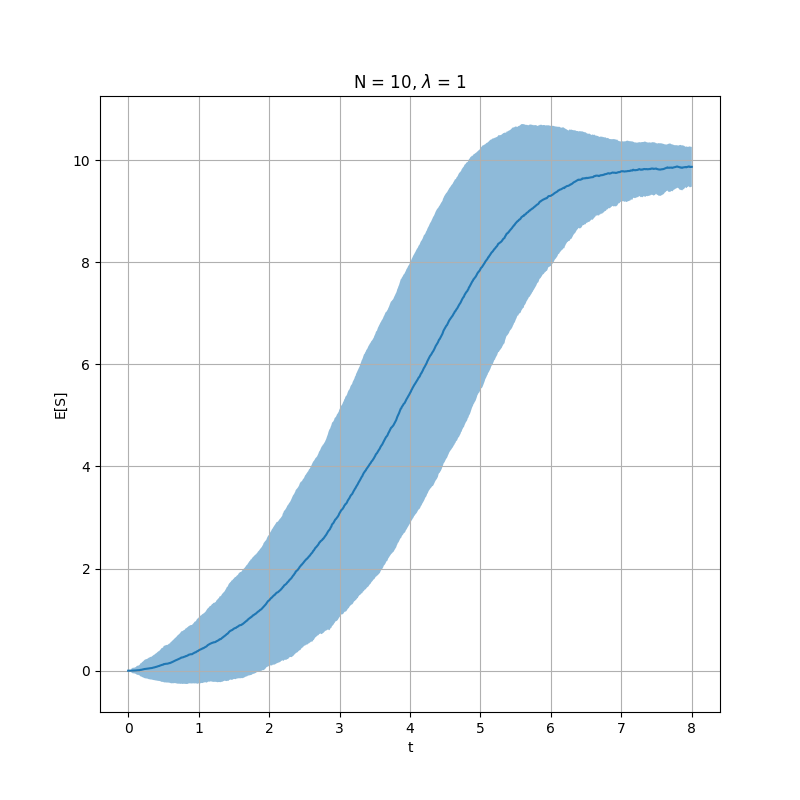
\includegraphics[width=0.8\textwidth, keepaspectratio]{../img/sampling/t_10_1.png}
				\caption{Численные решения для $ \phi(t) = t $}
			\end{figure}
		}
		
		\only<3>{
			% TODO обращаем внимание на фазовый переход, он есть!
			
			\begin{figure}
				\centering
				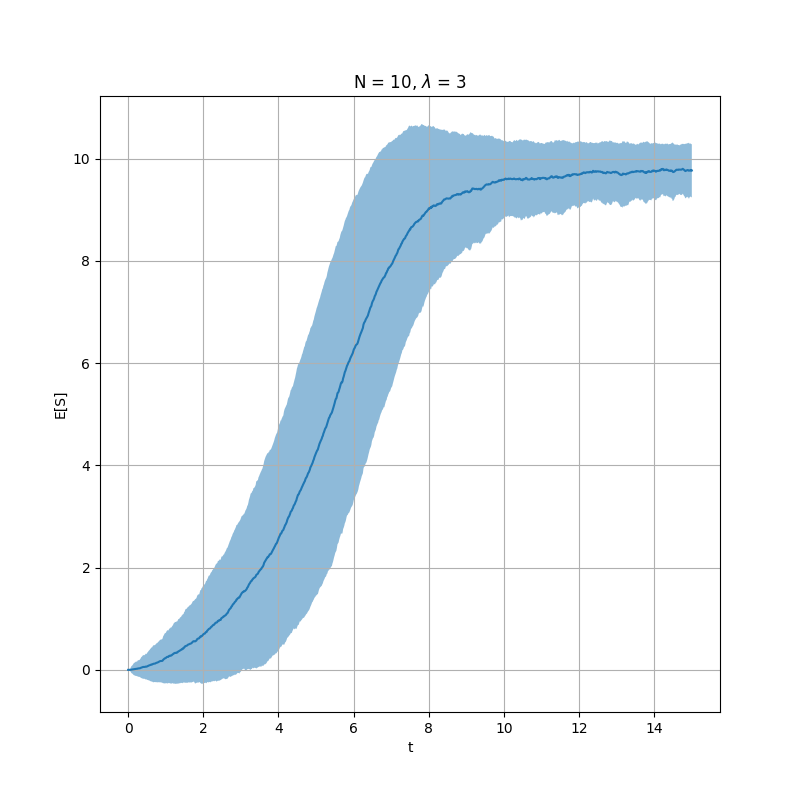
\includegraphics[width=0.8\textwidth, keepaspectratio]{../img/sampling/t_10_3.png}
				\caption{Численные решения для $ \phi(t) = t $}
			\end{figure}
		}
		
		\only<4>{
			% TODO обращаем внимание на фазовый переход, он есть!
			
			\begin{figure}
				\centering
				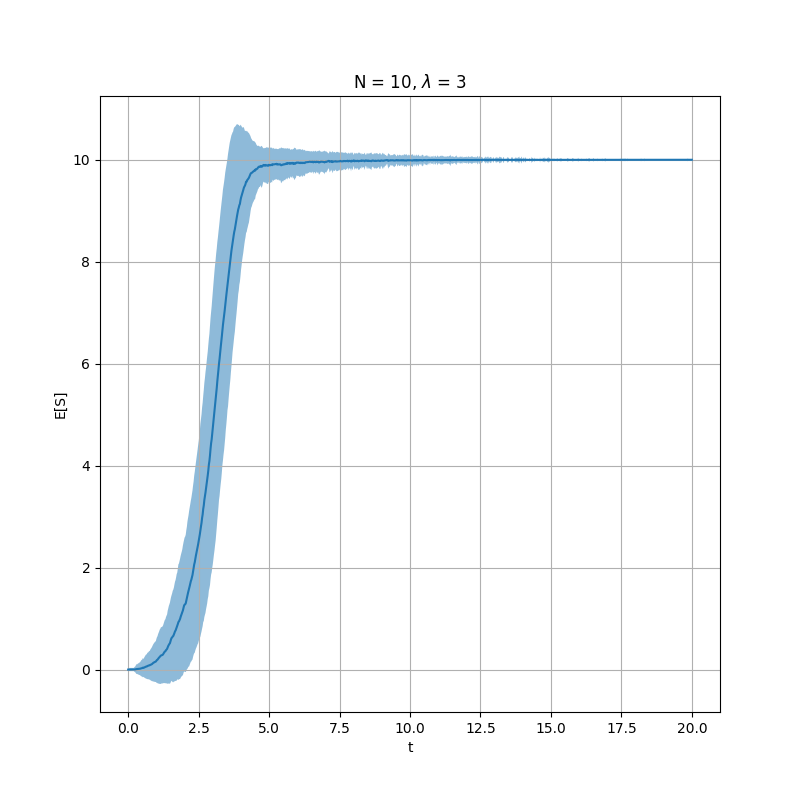
\includegraphics[width=0.8\textwidth, keepaspectratio]{../img/sampling/t^2_10_3.png}
				\caption{Численные решения для $ \phi(t) = t^2 $}
			\end{figure}
		}
		
		\only<5>{
			% TODO обращаем внимание на фазовый переход, он есть!
			
			\begin{figure}
				\centering
				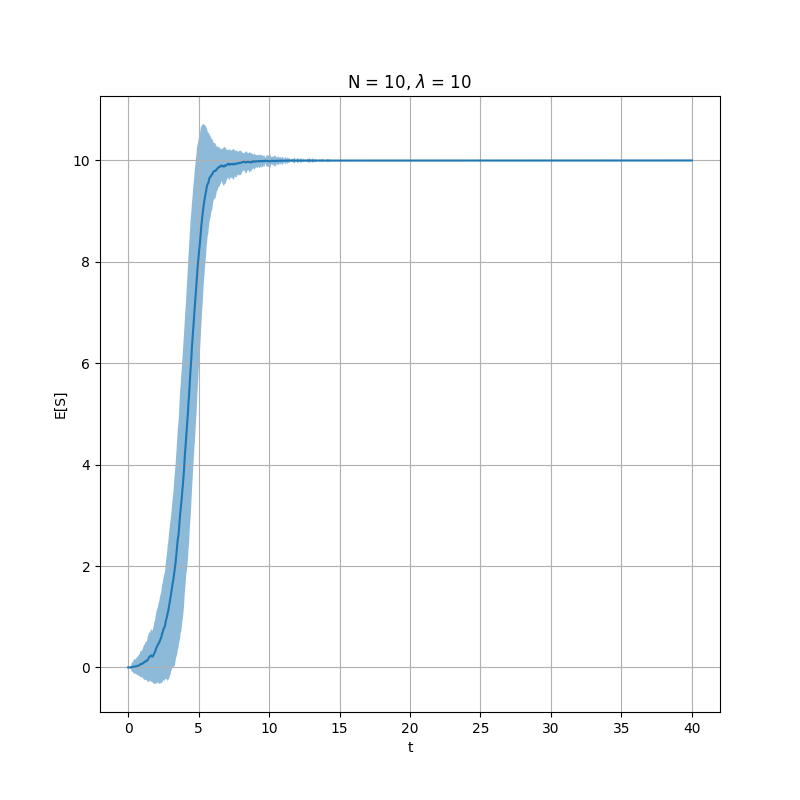
\includegraphics[width=0.8\textwidth, keepaspectratio]{../img/sampling/t^2_10_10.png}
				\caption{Численные решения для $ \phi(t) = t^2 $}
			\end{figure}
		}
		
		\only<6>{
			% TODO обращаем внимание на фазовый переход, он есть!
			
			\begin{figure}
				\centering
				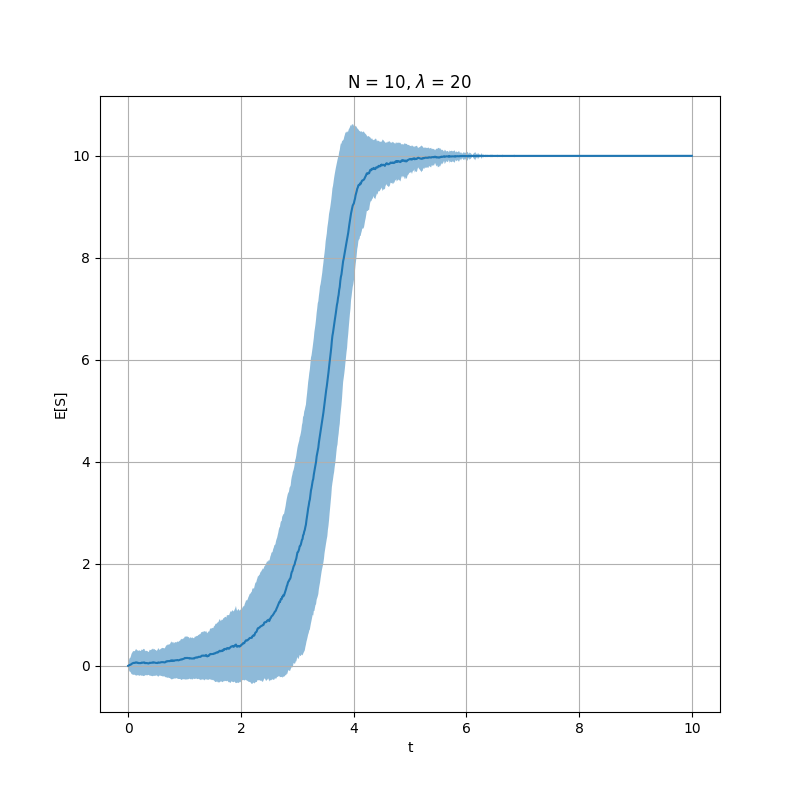
\includegraphics[width=0.8\textwidth, keepaspectratio]{../img/sampling/e^t_10_20.png}
				\caption{Численные решения для $ \phi(t) = \exp(t) $}
			\end{figure}
		}
		
	\end{frame}

	
	
\end{document}